\documentclass{article}

% if you need to pass options to natbib, use, e.g.:
%     \PassOptionsToPackage{numbers, compress}{natbib}
% before loading neurips_2026

% The authors should use one of these tracks.
% Before accepting by the NeurIPS conference, select one of the options below.
% 0. "default" for submission
% \usepackage{neurips_2026}
% the "default" option is equal to the "main" option, which is used for the Main Track with double-blind reviewing.
% 1. "main" option is used for the Main Track
%  \usepackage[main]{neurips_2026}
% 2. "position" option is used for the Position Paper Track
%  \usepackage[position]{neurips_2026}
% 3. "eandd" option is used for the Evaluations & Datasets Track
 % \usepackage[eandd]{neurips_2026}
% 4. "creativeai" option is used for the Creative AI Track
%  \usepackage[creativeai]{neurips_2026}
% 5. "sglblindworkshop" option is used for the Workshop with single-blind reviewing
% \usepackage[sglblindworkshop]{neurips_2026}
% 6. "dblblindworkshop" option is used for the Workshop with double-blind reviewing
\usepackage[dblblindworkshop]{neurips_2026}
% 7. "education" option is used for the Education Track
%  \usepackage[education]{neurips_2026}


% After being accepted, the authors should add "final" behind the track to compile a camera-ready version.
% 1. Main Track
 % \usepackage[main, final]{neurips_2026}
% 2. Position Paper Track
%  \usepackage[position, final]{neurips_2026}
% 3. Evaluations & Datasets Track
 % \usepackage[eandd, final]{neurips_2026}
% 4. Creative AI Track
%  \usepackage[creativeai, final]{neurips_2026}
% 5. Workshop with single-blind reviewing
%  \usepackage[sglblindworkshop, final]{neurips_2026}
% 6. Workshop with double-blind reviewing
%  \usepackage[dblblindworkshop, final]{neurips_2026}
% Note. For the workshop paper template, both \title{} and \workshoptitle{} are required, with the former indicating the paper title shown in the title and the latter indicating the workshop title displayed in the footnote.
% For workshops (5., 6.), the authors should add the name of the workshop, "\workshoptitle" command is used to set the workshop title.
% \workshoptitle{WORKSHOP TITLE}
% 7. Education Track
% \usepackage[education, final]{neurips_2026}

% "preprint" option is used for arXiv or other preprint submissions
 % \usepackage[preprint]{neurips_2026}

% to avoid loading the natbib package, add option nonatbib:
%    \usepackage[nonatbib]{neurips_2026}

\usepackage[utf8]{inputenc} % allow utf-8 input
\usepackage[T1]{fontenc}    % use 8-bit T1 fonts
\usepackage{hyperref}       % hyperlinks
\usepackage{url}            % simple URL typesetting
\usepackage{booktabs}       % professional-quality tables
\usepackage{amsfonts}       % blackboard math symbols
\usepackage{nicefrac}       % compact symbols for 1/2, etc.
\usepackage{microtype}      % microtypography
\usepackage{amsmath}
\usepackage{graphicx}
\usepackage{amsmath,amssymb}
\usepackage{bm} % optional; \boldsymbol from amsmath is used below

% Note. For the workshop paper template, both \title{} and \workshoptitle{} are required, with the former indicating the paper title shown in the title and the latter indicating the workshop title displayed in the footnote. 
\title{Sparse Scene Encoding with Foveated View Set Transformers}

% The \author macro works with any number of authors. There are two commands
% used to separate the names and addresses of multiple authors: \And and \AND.
%
% Using \And between authors leaves it to LaTeX to determine where to break the
% lines. Using \AND forces a line break at that point. So, if LaTeX puts 3 of 4
% authors names on the first line, and the last on the second line, try using
% \AND instead of \And before the third author name.


\author{%
  Emmanuel Daucé \\
  Institut de Neurosciences de la Timone\\
  Centrale Mediterranée\\
  Marseille, France \\
  \texttt{emmanuel.dauce@centrale-med.fr} \\
  % examples of more authors
  \And
  Laurent Perrinet \\
  Institut de Neurosciences de la Timone\\
  CNRS, Aix-Marseille Univ\\
  Marseille, France \\
  \texttt{laurent.perrinet@univ-amu.fr} \\
  % \AND
  % Coauthor \\
  % Affiliation \\
  % Address \\
  % \texttt{email} \\
  % \And
  % Coauthor \\
  % Affiliation \\
  % Address \\
  % \texttt{email} \\
  % \And
  % Coauthor \\
  % Affiliation \\
  % Address \\
  % \texttt{email} \\
}


\begin{document}


\maketitle


\begin{abstract}
  Standard self-supervised visual encoders produce feature vectors that are rich in semantic content but largely devoid of spatial information: shifted views of the same scene are trained to yield near-identical representations, erasing the very information needed to recover their relative position. This paper studies self-supervised representations learned from foveated visual inputs, where high resolution is restricted to the center of each view. We show that combining a forward model, predicting the representation of a target view from the current view and a motor command, with an inverse model, recovering that command from a pair of representations, is enough to force latent representations to re-integrate spatial content. The resulting description is equivariant rather than invariant, without requiring any explicit geometric constraint on the embedding space. Crucially, this spatial component can be added to an already pretrained encoder through fine-tuning alone, without destroying the content already encoded: label information is largely preserved throughout the procedure. Once present, this spatial content supports powerful predictive mechanisms: a target feature vector, or ``query'', can be used to direct attention toward specific regions of a scene, effectively building a predictive, content-addressable map from a single view. We further propose representing a scene not as a single dense descriptor, but as a sparse set of such view vectors, motivated by considerations of biological plausibility. This sparse view-set is cheap to store, requiring only a handful of vectors per scene, which makes it a natural candidate both for embedded systems operating under tight memory constraints and for the compressed encoding of past saccades presumably maintained by biological visual systems.
\end{abstract}

\section{Introduction}

In the field of artificial vision, numerous studies have sought to establish correspondences between the processing of the visual field as it is projected onto the retina and the successive processing stages in the cortex~\cite{hubel1962receptive,felleman1991distributed,fukushima1980neocognitron,yamins2014performance,yamins2016using}, revealing genuine convergences, from the elementary processing of oriented filters to the more global integration of the objects contained in the scene~\cite{zeiler2014visualizing,guclu2015deep,cichy2016comparison,eickenberg2017seeing,khaligh2014deep,schrimpf2020integrative}. These results, however, only reflect superficial similarities~\cite{geirhos2019imagenet,bowers2023deep}, and cannot explain the unified percept produced by interpreting and understanding the spatial organization of a scene viewed through a sequence of saccades~\cite{melcher2008transsaccadic}. 

Looking at the image processing literature on one hand and the neuroscience literature on the other, one may rather consider a \emph{divergence} of representations rather than a convergence once the visuo-motor system is taken into account.
Indeed, image processing operates on complete scenes made up of regular pixel grids (images or videos), and the pixel data is processed in parallel at the patch level, either through progressive pooling (CNNs~\cite{lecun1998gradient,krizhevsky2012imagenet}) or through tokens (ViTs~\cite{dosovitskiy2021image}). This is very far from human visual processing, which relies on an anisotropic retina made of a central fovea of very high resolution and peripheral regions of low resolution~\cite{curcio1990human}. Human visual processing is also sequential: the eye performs saccades, sampling specific points of the scene~\cite{yarbus1967eye,findlay2003active}. Since the two visual systems differ, one may expect the representation of space, and of relative positions or distances, to differ as well. Indeed, most spatial processing (the relative position of objects) in artificial systems relies on dense representations, such as those obtained at the output of a DINO or ViT model~\cite{caron2021emerging,oquab2024dinov2}, which preserve the geometry of the original image. Representing space in a human (or primate) visual system is a much harder problem. There is no reference grid, and all (relative) position information must rely on the eye's own movements (ego-motion), that is, on saccade motor commands (corollary discharge)~\cite{duhamel1992updating,sommer2002pathway,wurtz2008neuronal}, and/or on an understanding of the scene geometry. Foveated and glimpse-based artificial models have started to explore this regime~\cite{mnih2014recurrent,cheung2016emergence,dauce2018active,dauce2020dual,jeremie2026foveated,ghaemi2026seq,immonen2026action}.

This fundamental structural difference partly explains the well-known weakness of artificial vision models at interpreting the geometry of the images they process~\cite{kamath2023whatsup,tong2024eyes}. Visual recognition models excel at identifying object labels from elaborate statistics on the relative distribution of shapes and textures~\cite{geirhos2019imagenet,baker2018deep}, but appear to fail at interpreting the distances, positions and relative sizes of the objects that compose the scene. This problem of geometric reconstruction has already been addressed in several ways. Capsule networks are a notable example, as they explicitly frame the problem as one of inverse graphics~\cite{hinton2011transforming,sabour2017dynamic,kulkarni2015deep}. More recent models from the self-supervised learning (SSL) family tackle the problem by adding geometric constraints directly within the embedding space~\cite{bardes2022vicregl}, or, more simply, through forward prediction  \cite{dangovski2022equivariant,garrido2023sie}. Finally, ``world models'' rely on predictive (causal) models trained on video data, operating within the embedding space itself, with strong regularization constraints to prevent representation collapse~\cite{ha2018world,lecun2022path,assran2023ijepa,bardes2024vjepa,balestriero2025lejepa}.

The question of how space is represented in such active vision systems then arises naturally~\cite{bajcsy1988active,ballard1991animate}. The hypothesis we formulate, and seek to test with our model, is that in the absence of absolute reference, the scene recognition system needs to integrate some ego-motion features in its internal representations in order to correctly appreciate the spatial relations within the visual scene.  This is consistent with the embodied cognition tradition, which holds that spatial content is grounded in sensorimotor contingencies rather than extracted from a static image alone~\cite{oregan2001sensorimotor}. This view is moreover supported both by neurophysiological evidence that gaze and movement related signals shape spatial encoding in parietal cortex~\cite{andersen1985encoding,crapse2008corollary}, and by machine learning work showing that ego-motion  alone can serve as self-supervised signal for effective visual prediction~\cite{jayaraman2015learning,agrawal2015learning}. 
More precisely, we exploit here the decorrelation property of foveal vision to implement effective equivariance learning in transformers, through keeping essential scene content information, with the help of a predictor and an inverse model operating in the representation space.

\section{Model}

\begin{figure}[t]
  \centering
  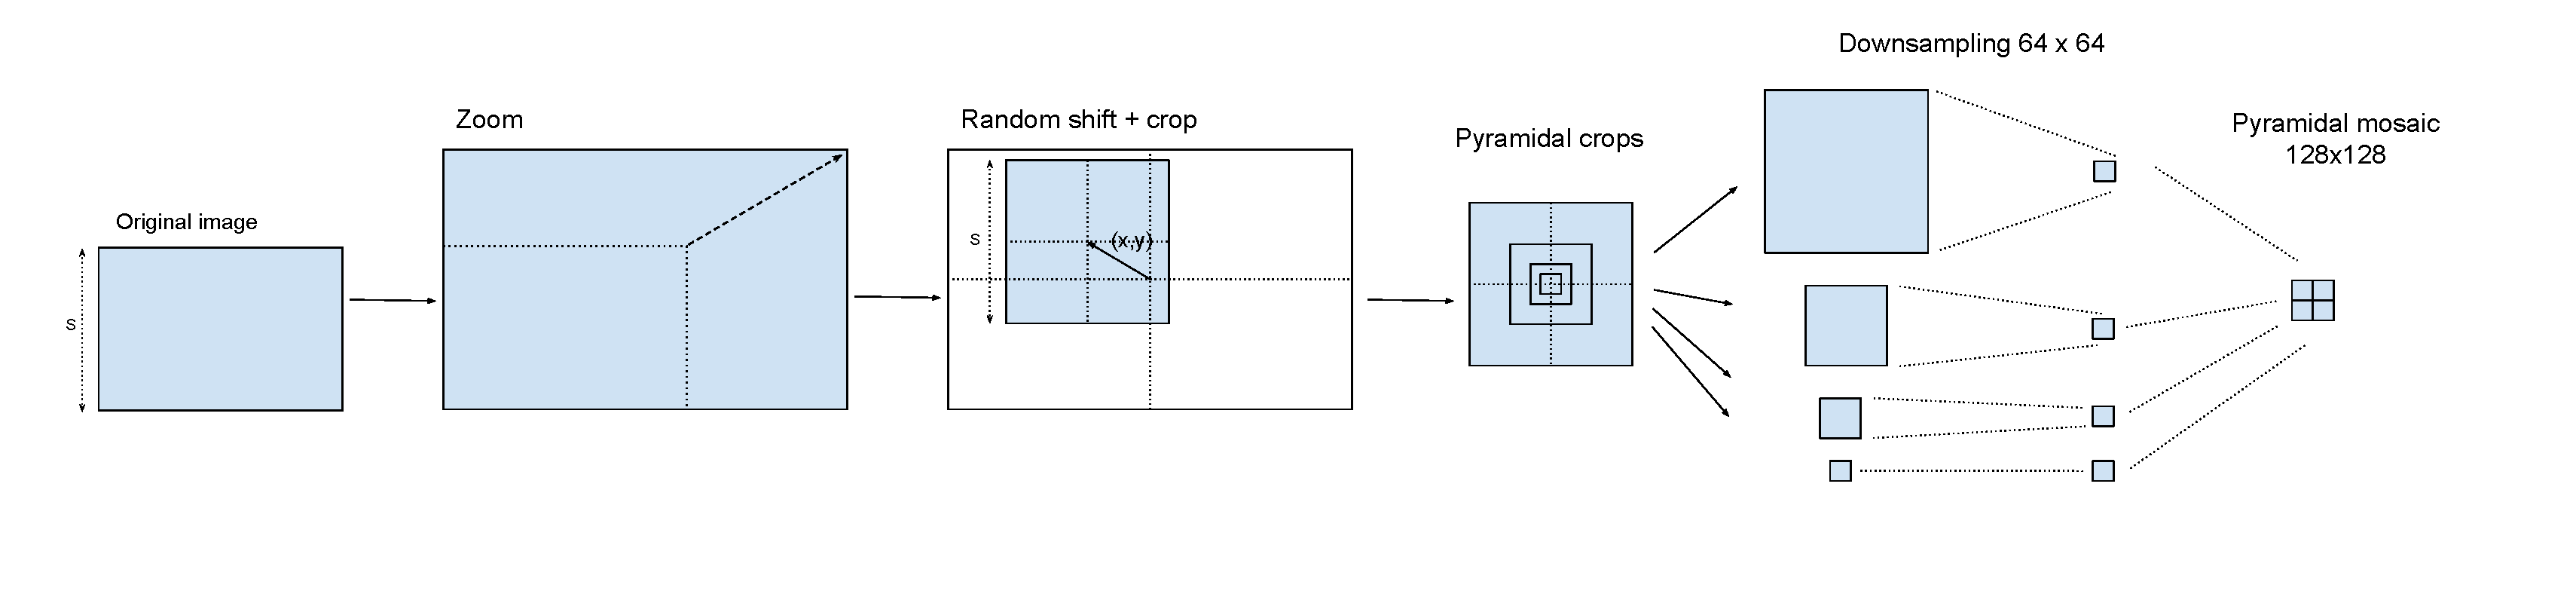
\includegraphics[width=\linewidth]{figs/01_pipeline.pdf}
  \caption{\textbf{Generation of foveated input views.}
  The input views are obtained through a random transformation of the input image, corresponding to a partial view randomly shifted away from the center.
  This transformation consists in:
  (1) zooming in on the image, from size $H \times W$ to size $H_z \times W_z$ (in pixels), using bicubic interpolation;
  (2) drawing a random position $(x,y)$ from a 2D Gaussian distribution with standard deviation $\sigma$;
  (3) defining a reference size $S = \min(H, W)$ and a zoomed size $S_z = \min(H_z, W_z)$, in pixels. The center of the zoomed image is $\left(\frac{H_z}{2}, \frac{W_z}{2}\right)$, and the center of the sample is shifted from it as
  $c = (c_x, c_y) = \left(\frac{H_z + S_z x}{2}, \frac{W_z + S_z y}{2}\right)$;
  (4) cropping the image horizontally between $c_x - \frac{S}{2}$ and $c_x + \frac{S}{2}$, and vertically between $c_y - \frac{S}{2}$ and $c_y + \frac{S}{2}$, with mirror padding.
  The resulting image is a square image of size $(S,S)$, corresponding to a ``view'' shifted from the initial center of the image.
  A second transformation is then applied to simulate foveal vision around the center. For our experiments, we use a ``pyramidal'' transformation as defined by Geisler and Perry~\cite{geisler1998real}, with four resolution levels.
  To this end:
  (1) denoting by $c$ the center of the image, we define four crop levels: for $k \in \{1, 2, 4, 8\}$, the crops are
  $\left(c_x - \frac{S}{2k},\, c_x + \frac{S}{2k},\, c_y - \frac{S}{2k},\, c_y + \frac{S}{2k}\right)$;
  (2) each cropped image is resized to $64 \times 64$ pixels by bicubic interpolation;
  (3) the four images are concatenated into a $128 \times 128$ pixel mosaic.
  The final image therefore contains visual information at high resolution in the center (the square corresponding to the smallest crop) and at low resolution in the periphery (the whole image downsampled to $64 \times 64$), with two intermediate resolution levels.}
  \label{fig:foveated-views}
\end{figure}

The model we propose is deliberately simple, yet sufficiently expressive to address our question.
It builds on a DINO-pretrained visual transformer~\cite{caron2021emerging,oquab2024dinov2}, fine-tuned within a student--teacher predictive scheme with a slowly updated (EMA) teacher~\cite{grill2020bootstrap}, where a predictor conditioned on the motor command anticipates the representation of the next view in embedding space, and where an inverse model recovering the action from a pair of views prevents representation collapse~\cite{agrawal2015learning,pathak2017curiosity}.

\begin{figure*}[t]
  \centering
  \begin{minipage}[c]{0.59\linewidth}
    \centering
    \textbf{(A)}\\[2pt]
    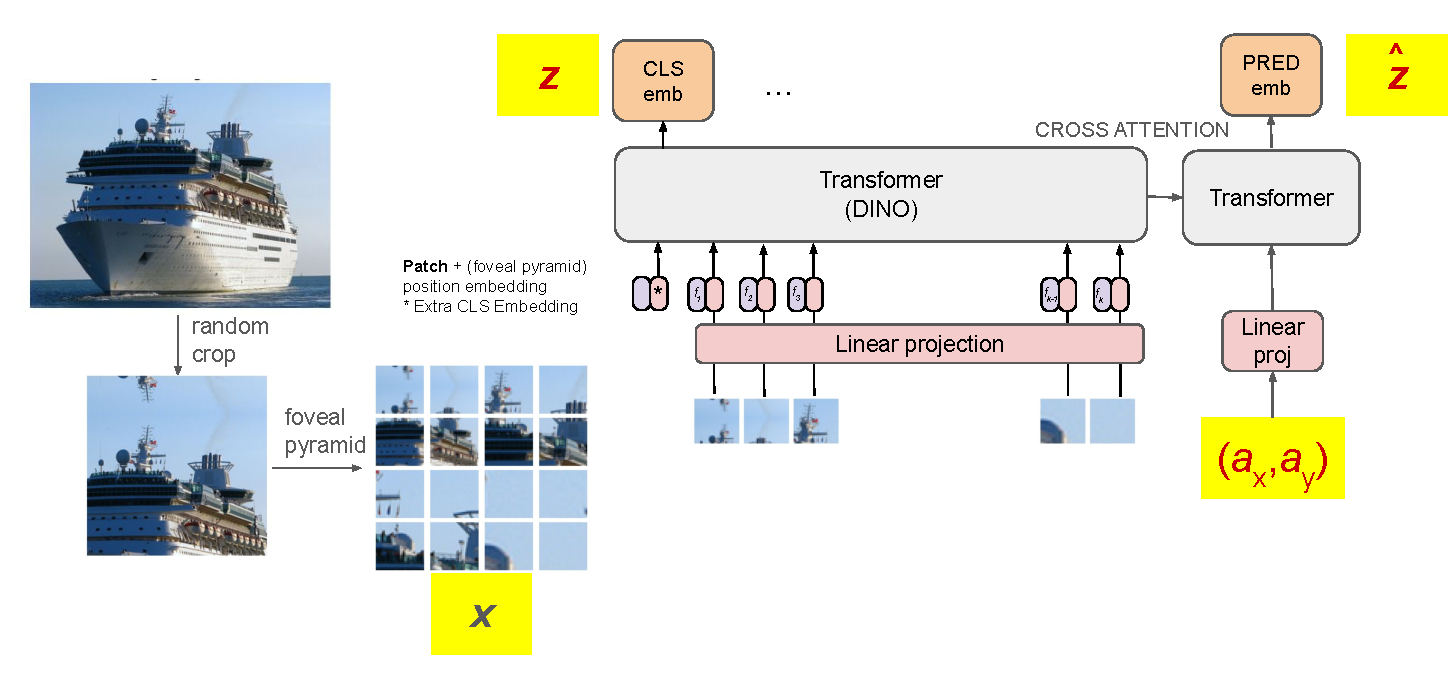
\includegraphics[width=\linewidth]{figs/02_1_predictor.pdf}
  \end{minipage}\hfill
  \begin{minipage}[c]{0.39\linewidth}
    \centering
    \textbf{(B)}\\[2pt]
    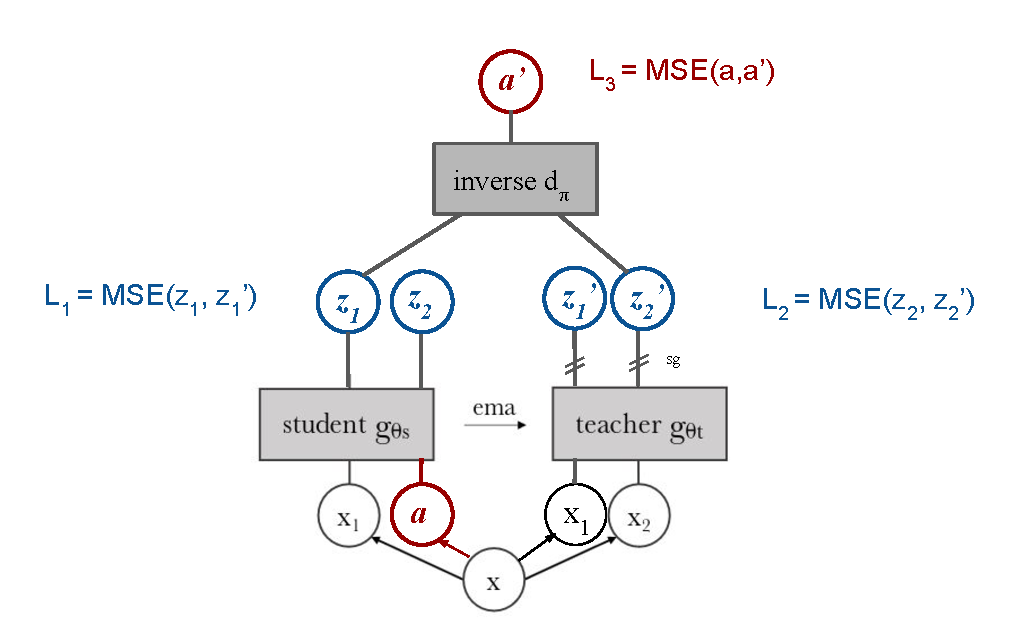
\includegraphics[width=\linewidth]{figs/02_2_training.pdf}
  \end{minipage}
  \caption{\textbf{Predictive model and training pipeline.}
  \textbf{(A)} The predictive model takes as input a pyramidal view $\boldsymbol{x}$ of size $128 \times 128$. This view is split into $8 \times 8$ patches, which are flattened and linearly projected as input to a pretrained DINO~v1 transformer~\cite{caron2021emerging} (\texttt{vit\_base\_patch8\_224.dino}, 12 transformer blocks, token dimension 768), resulting in a total of $16 \times 16$ input patches plus the CLS token. An ad-hoc positional embedding is added, obtained by linearly combining DINO's positional encodings at the positions of the patches \emph{within} the foveal pyramid.
  The input of the predictor is the 2D displacement command $(a_x, a_y)$, followed by a linear projection. The predictor uses the same 12-block architecture, with cross-attention over the tokens of the visual input.
  The two outputs considered are the [CLS] token, $\boldsymbol{z}$, and the predictor output token [PRED], $\hat{\boldsymbol{z}}$.
  \textbf{(B)} Training follows the student--teacher scheme defined in~\cite{grill2020bootstrap,caron2021emerging}. A training example is a triplet $(\boldsymbol{x}_1, \boldsymbol{x}_2, \boldsymbol{a})$, where $\boldsymbol{x}_1$ and $\boldsymbol{x}_2$ are foveal views and $\boldsymbol{a}$ is the displacement of the eye between the two views. The student uses $\boldsymbol{x}_1$ and $\boldsymbol{a}$ to predict the representations $\boldsymbol{z}_1$ and $\boldsymbol{z}_2$, following the predictive architecture defined in panel~(A). The teacher uses the inputs $\boldsymbol{x}_1$ and $\boldsymbol{x}_2$ to generate $\boldsymbol{z}_1'$ and $\boldsymbol{z}_2'$. Consistency with the learned representations is enforced by the similarity between the \emph{unnormalized} $\boldsymbol{z}_1$ and $\boldsymbol{z}_1'$ (MSE loss), while the training of the predictor relies on the similarity between $\boldsymbol{z}_2$ and $\boldsymbol{z}_2'$. Finally, the spatial consistency of the representations is enforced by the inverse model, a 3-layer MLP preceded by a normalization layer (LayerNorm)~\cite{ba2016layer}, which partly mitigates the risk of collapse. Collapse is also prevented by using different learning rates across the network layers: $\alpha_\text{DINO backbone}=10^{-6} < \alpha_\text{predictor}=10^{-5} < \alpha_\text{inverse model}=10^{-4}$. The prediction $\boldsymbol{a}'$ is compared to $\boldsymbol{a}$ with an MSE loss. Only the student weights are trained (stop-gradient on the teacher). The teacher weights are updated as an exponential moving average (EMA)  of the student weights (momentum 0.9999).
  To generate the views, the zoom is set to 1.5.
  A \emph{curriculum learning} principle~\cite{bengio2009curriculum} is applied during training, with a progressively increasing shift between views, drawn from a Gaussian distribution whose standard deviation increases linearly from 0.07 to 0.3.
  Training uses the AdamW optimizer~\cite{loshchilov2019decoupled}, bfloat16 autocast and gradient norm clipping, on ImageNet-1k~\cite{russakovsky2015imagenet}, for 20 epochs, with image batchs of size 64.}
  \label{fig:model-training}
\end{figure*}

At the core of the system are two views, $\boldsymbol{x}_1$ and $\boldsymbol{x}_2$, of the same scene (see fig~\ref{fig:shift-comparison}, left panel). These are foveal views, with only low spatial frequencies in the periphery (see figures~\ref{fig:foveated-views} and \ref{fig:attn-comparison}). We essentially consider the [CLS] token output vector of a DINO-type architecture~\cite{caron2021emerging}, which concentrates the description of a view. The two views (initial and final) are interpreted as a 2D shift of the ``eye'', which we implement with the coordinates $(a_x,a_y)$ in our setup, but which can more generically be regarded as a motor command $\boldsymbol{a}$ (or as ego-motion). The spatial ``relation'' between the two views is thus $\boldsymbol{a}$, and conversely any pair of views should in principle allow one to deduce the command that produced them (provided the inverse model is actually invertible~\cite{wolpert1998multiple,agrawal2015learning}). In an SSL context, we are interested in the induced latent representations. Let $\boldsymbol{z}_1$ and $\boldsymbol{z}_2$ be the representations of $\boldsymbol{x}_1$ and $\boldsymbol{x}_2$. 
Space, understood as a relation between views, then amounts to the existence of latent representations $\boldsymbol{z}_1$ and $\boldsymbol{z}_2$ rich enough for the action $\boldsymbol{a}$ to be reconstructed by the inverse model.

The principal component of the model is the predictor (see figure~\ref{fig:model-training}A). The predictor is a cross-attention layer running in parallel to the DINO/vision transformer architecture~\cite{dosovitskiy2021image,jaegle2021perceiver}, which takes as input a token obtained by a linear projection of $(a_x,a_y)$ toward the embedding space (of dim. 768). Yet we remain within a self-supervised logic since no label is involved here. The model thus performs a dual computation: encoding its own view $\boldsymbol{x}_1 \rightarrow \boldsymbol{z}_1$ through the main transformer pathway and predicting the future representation $\boldsymbol{x}_1, \boldsymbol{a} \rightarrow \boldsymbol{z}_2$ through the predictor pathway, in the spirit of joint-embedding predictive architectures~\cite{assran2023ijepa,bardes2024vjepa}. Once trained, this component will make it possible to build a predictive map from the current view, using a simple grid of coordinates as input (see Section~\ref{sec:prediction-map}). 

\begin{figure}[t]
  \centering
  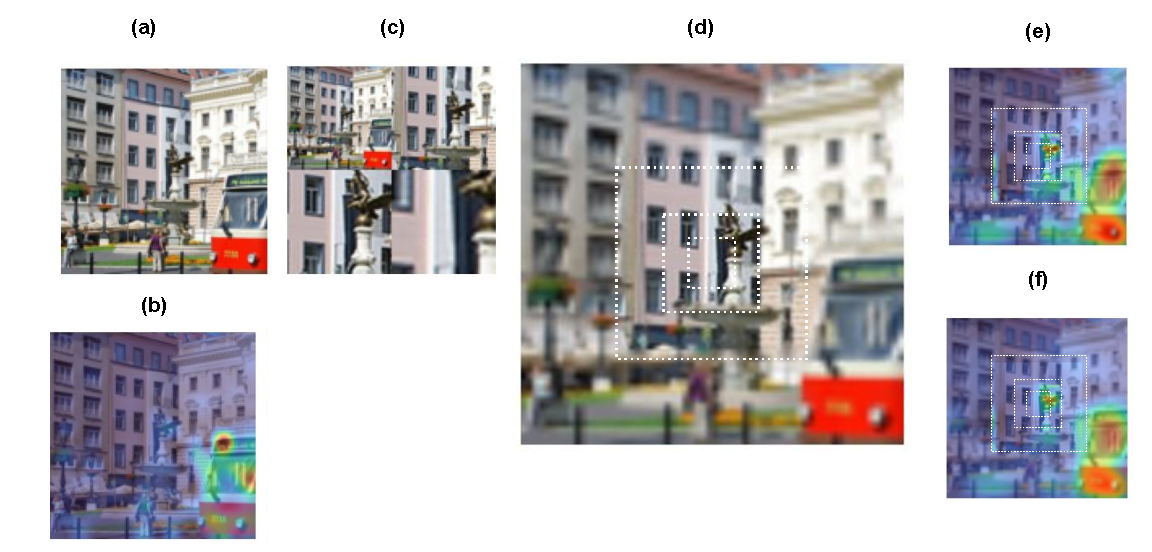
\includegraphics[width=0.7\linewidth]{figs/03_attn-maps.pdf}
  \caption{\textbf{Comparison of attention maps}. Different inputs, taken from a same photograph, are considered. Panel (a) : a crop of the original scene, downsampled to $128\times128$ pixels, is sent to the model. Panel (b) overlays the average attention map of the CLS token at the last block. Panel (c): the same image zone is transformed according to the pyramidal/foveal approach, i.e., built from four nested sub-images. Panel (d) shows the reconstruction, in standard Cartesian space, of the visual information content (i.e. sharp at the center, blurred in the periphery). The reconstructed attention map of the last block is shown before fine-tuning (panel (e)), and after fine-tuning (panel (f)).}
  \label{fig:attn-comparison}
\end{figure}

The structuring element of our architecture is the inverse model $\boldsymbol{z}_1, \boldsymbol{z}_2 \rightarrow a$, which encourages the internal representations (the current and predicted representations) to retain positional information in order to do the prediction.
We therefore expect the encodings of these two views to be expressive enough for their spatial relation to be extractible. 

Training requires a student and a teacher~\cite{grill2020bootstrap,caron2021emerging}. It relies on triplets $(\boldsymbol{x}_1, \boldsymbol{x}_2, \boldsymbol{a})$, where $\boldsymbol{a}$ is a relative displacement and $\boldsymbol{x}_1, \boldsymbol{x}_2$ are the corresponding views. The student is the predictor: it encodes $\boldsymbol{x}_1 \rightarrow \boldsymbol{z}_1$ and predicts $\boldsymbol{z}_2$ from $\boldsymbol{a}$. The teacher encodes $\boldsymbol{x}_1 \rightarrow \boldsymbol{z}_1'$ and $\boldsymbol{x}_2 \rightarrow \boldsymbol{z}_2'$, and the similarities $\mathrm{sim}(\boldsymbol{z}_1,\boldsymbol{z}_1')$ and $\mathrm{sim}(\boldsymbol{z}_2,\boldsymbol{z}_2')$ are used jointly as the loss function. In complement, the inverse model is trained on $(\boldsymbol{z}_1, \boldsymbol{z}_2') \rightarrow a$ (see figure \ref{fig:model-training}B), allowing the gradient to backpropagate through the DINO weights, but preventing any information leak through the predictor pathway. In practice, we apply the method on a DINO-pretrained teacher with a rather slow exponential moving average (EMA) to maintain the expressivity of the internal DINO representations.

%\begin{figure}[t]
%  \centering
%  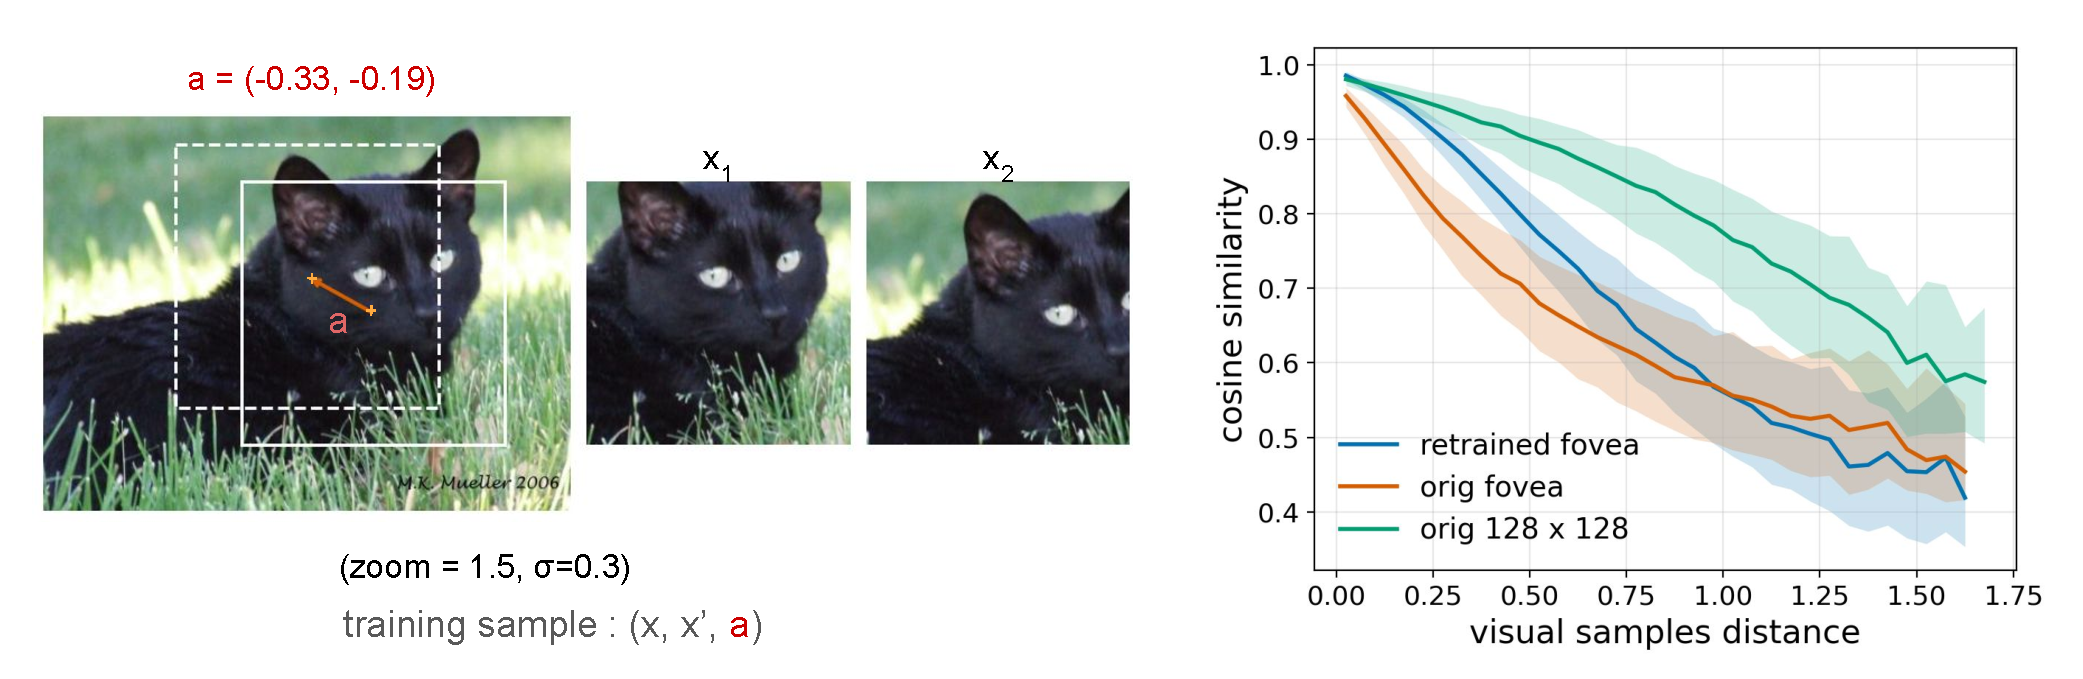
\includegraphics[width=\linewidth]{figs/04_shift_comparison.pdf}
%  \caption{\textbf{Shift comparison}. At the core of the self-supervised learning algorithm are the two views of a same scene : $\boldsymbol{x}_1$ and $\boldsymbol{x}_2$. Each view is characterized by its own (normalized) coordinates (in $[-1,1]$), and their relative shift, noted $a_x$ and $a_y$, reflects the eye "movement" over the whole scene. A training sample is thus composed of a triplet ($\boldsymbol{x}_1,\boldsymbol{x}_2,\boldsymbol{a}$)}. On the right figure, we show the cosine similarity between view encodings, as a function of the distance.
%\end{figure}

\begin{figure}[t]
  \centering
  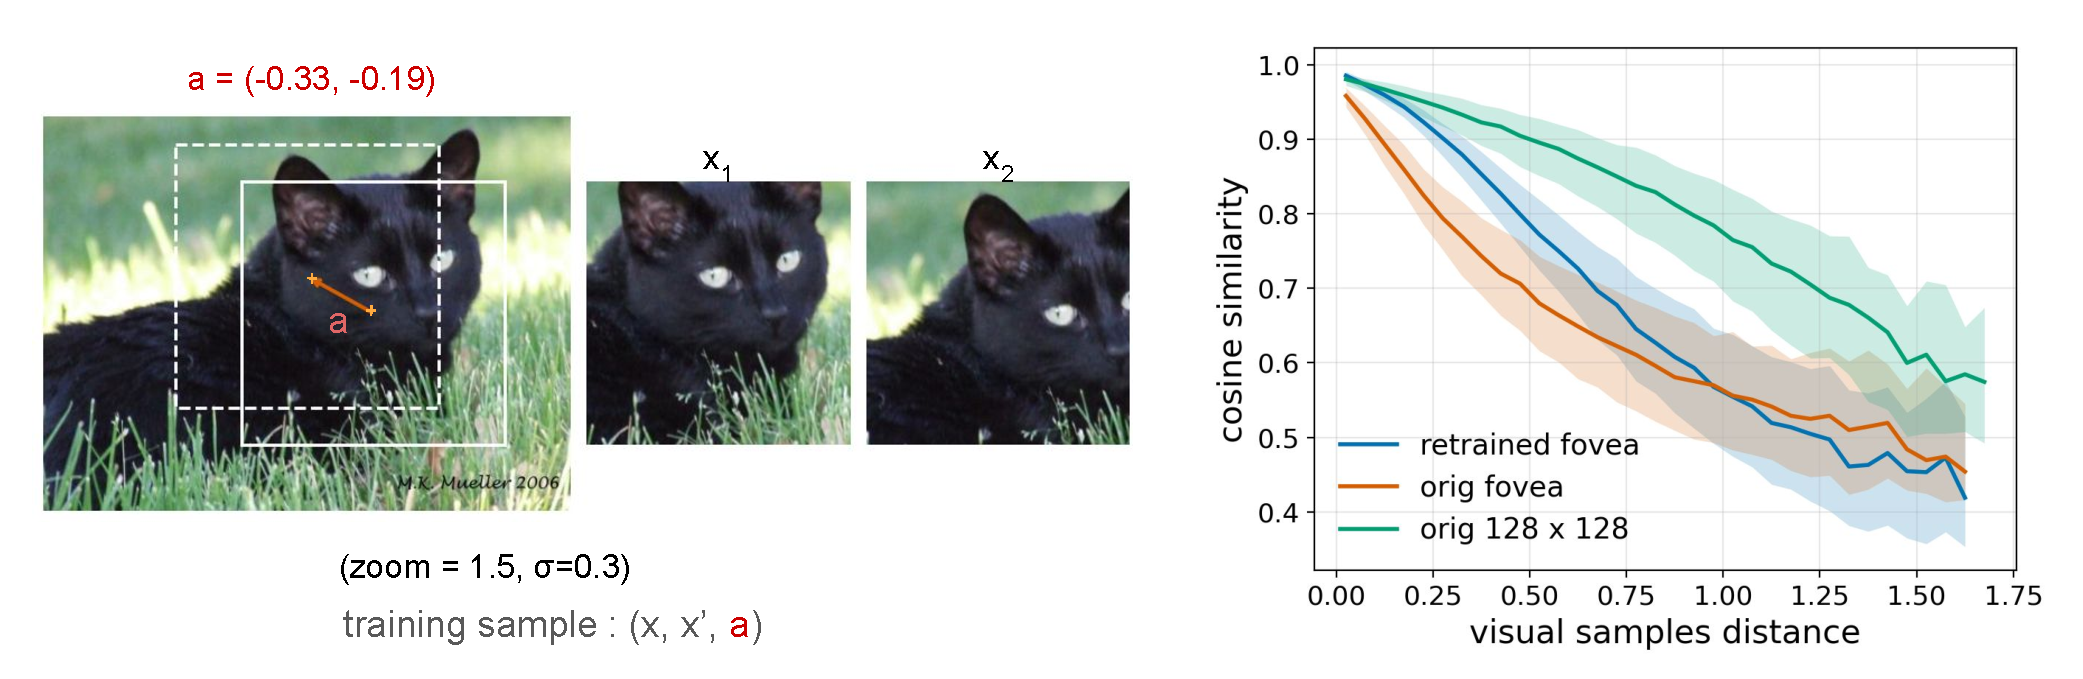
\includegraphics[width=\linewidth]{figs/04_shift_comparison.pdf}
  \caption{\textbf{Shifted images comparison}. At the core of the self-supervised learning algorithm are two views of the same scene, $\boldsymbol{x}_1$ and $\boldsymbol{x}_2$. Each view is characterized by its own (normalized) coordinates (in $[-1,1]$), and their relative shift, denoted $a_x$ and $a_y$, reflecting the eye ``movement'' across the whole scene. A training sample is thus composed of a triplet $(\boldsymbol{x}_1,\boldsymbol{x}_2,\boldsymbol{a})$. These views are encoded by a transformer, and the encoding is read out from the [CLS] token for several models: we compare, on the right-hand panel, a standard DINO model with $128\times128$-pixel inputs (green), a DINO model with foveal inputs (orange), and a DINO model with foveal inputs fine-tuned by our method (blue). We then measure in the representation space the similarity between the representations, as a function of the (normalized) distance between the views, averaged over random spatial shifts over the ImageNet-1K test set.}
  \label{fig:shift-comparison}
\end{figure}

\begin{figure}[t]
  \centering
  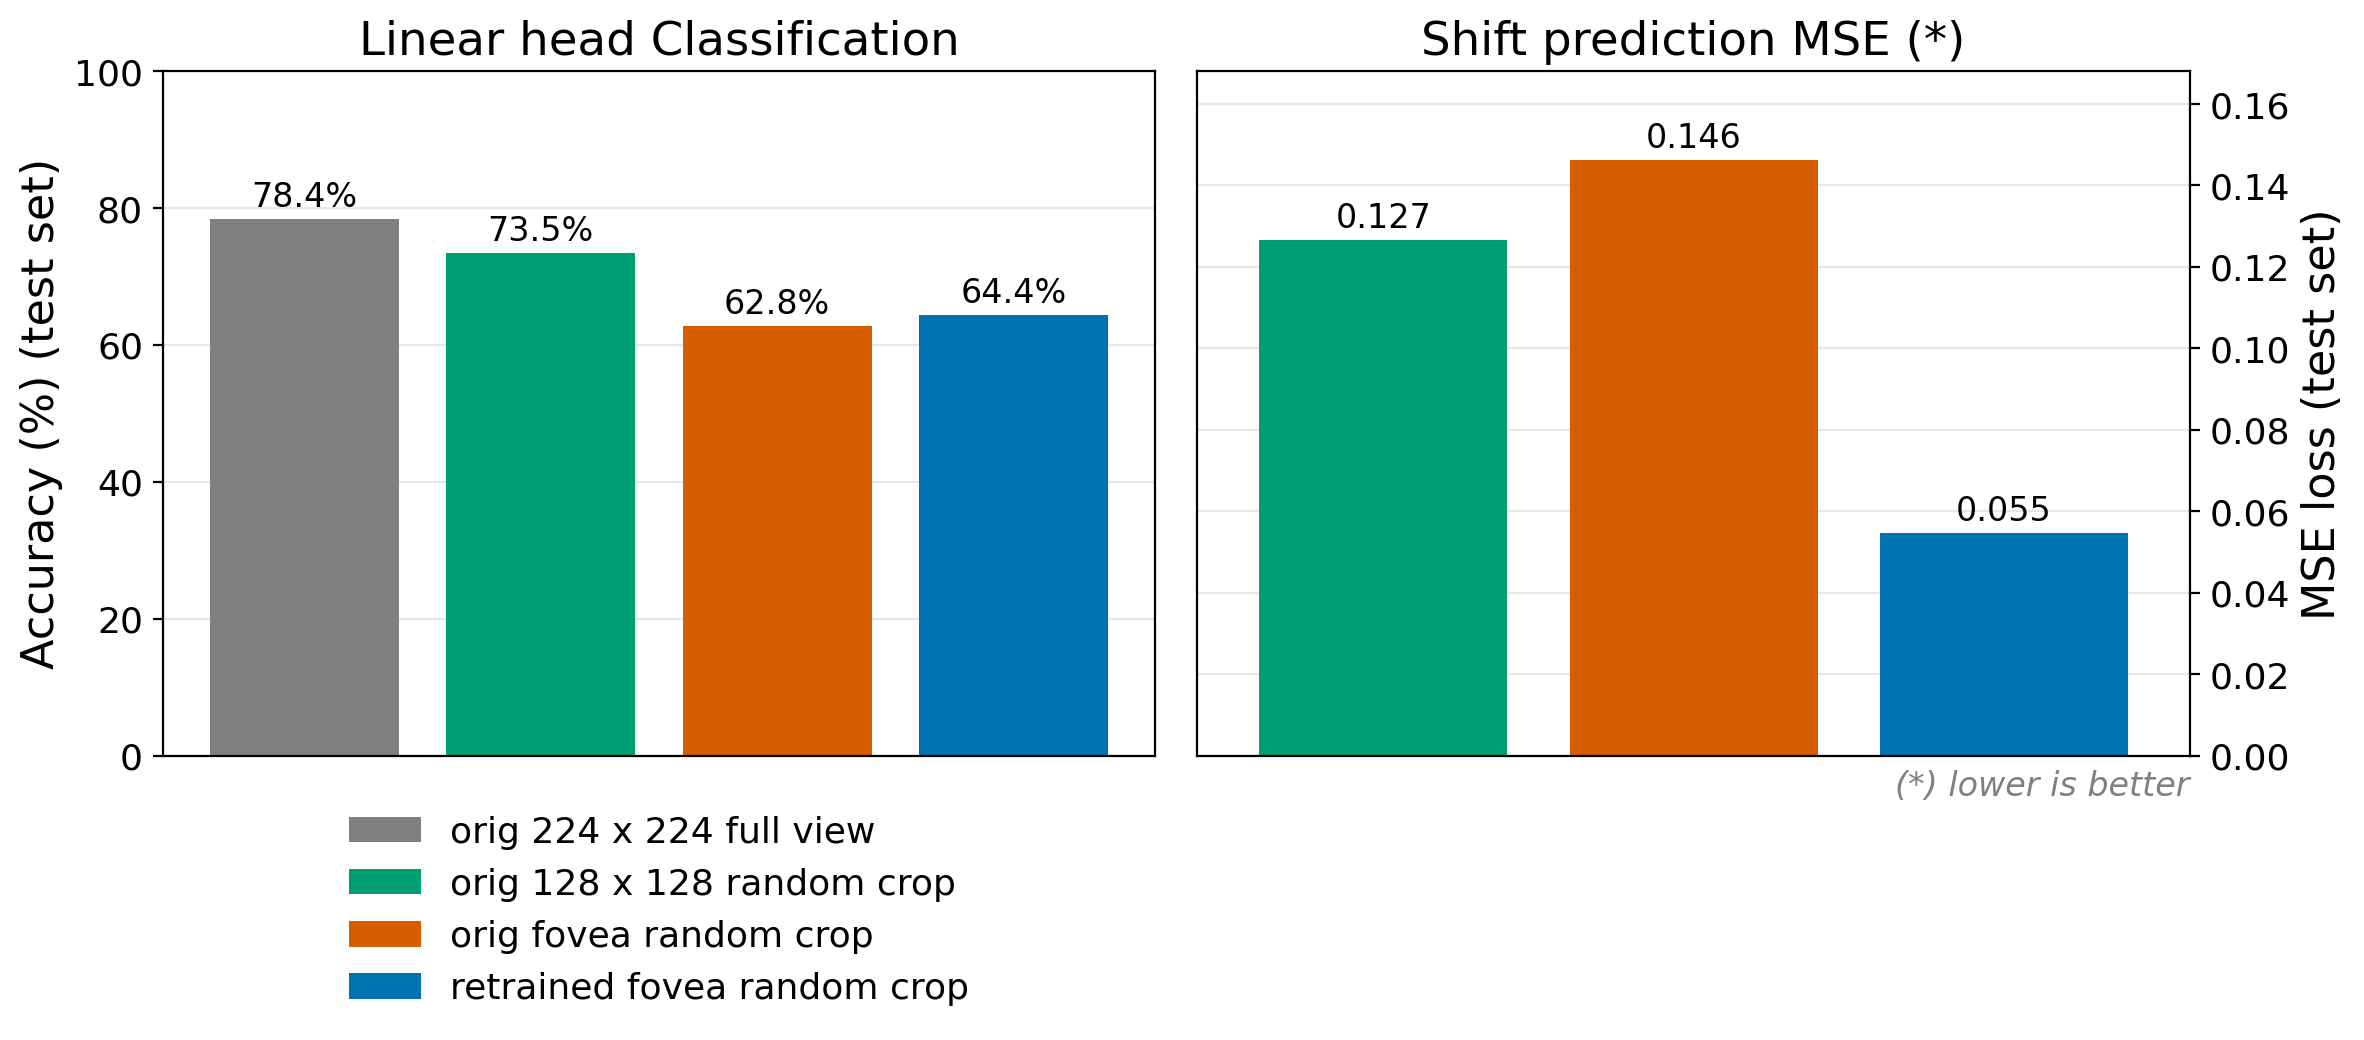
\includegraphics[width=.7\linewidth]{figs/05_classif_and_shift.png}
  \caption{\textbf{Classification and shift prediction}.  The left panel shows the classification accuracy on the test set for the original DINO1-224-patch8 model with the full image as input, the standard model with random $128\times128$ crops, the non-fine-tuned foveal model, and the fine-tuned foveal model. Training runs for 20 epochs, with a 5-epoch linear warmup followed by cosine annealing, using SGD with momentum 0.9. The right panel shows the mean squared error of the predicted spatial shift between view 1 and view 2, from the transformer's internal representations, for standard $128\times128$ crops, and for foveal inputs on the non-fine-tuned and fine-tuned models. Training runs for 100 epochs, with a 16-epoch linear warmup followed by cosine annealing, using the AdamW optimizer.}
  \label{fig:classif-and-shift}
\end{figure}

\section{Results}


\subsection{Attention maps}
It is important to understand the effect of the foveal deformation on the internal representations of the transformer. The foveal mosaics, of size $128 \times 128$ pixels, are more ``compressed'', and have a different spatial organization than the images that were used during the initial training of DINO~\cite{caron2021emerging}. The positional encodings were therefore reconstructed by interpolation~\cite{dosovitskiy2021image}. As an illustration, fig~\ref{fig:attn-comparison} compares the average attention maps at token [CLS] in the last block of the transformer, before and after fine-tuning, on foveal inputs and on a standard input (city scene). Those maps appear consistent across visual modalities. Similar regions (e.g. bus and central pedestal) attract the majority of spatial attention, regardless of whether the visual input is plain or foveal. Interestingly, peripheral regions (pedestrians, bollards) attract part of the spatial attention for the standard input, whereas these same regions remain essentially blurred and indistinct for the foveal ones.

\subsection{Representation analysis}

Let us now consider the feature vectors read at the output of the [CLS] token pathway, and compare their spatial diversity across visual modalities. The right panel of fig~\ref{fig:shift-comparison} gives an intuition of this diversity by measuring the cosine similarity between two spatially-shifted representations extracted from the same image (the lower the cosine similarity, the higher the spatial diversity). The standard visual inputs (resized to $128\times128$) are compared with the foveal ones, before and after fine-tuning. As expected, the similarity between representations decreases with the spatial distance between them, but this decrease is much steeper for foveal inputs. A persistence of cosine similarity at large distances reflects a form of spatial \emph{invariance}, a property that is encouraged in DINO's setup. By altering the underlying geometry, our foveal input sharply reduces this spatial invariance, providing fertile ground for equivariant representations. After fine-tuning, we observe however a slight reversal of this trend, with a somewhat slower decay, indicating that the learned representations capture longer-range information.

Another way to compare the expressiveness of the transformer's output representation is to train linear or MLP heads on specific tasks. We train (1) a linear head on ImageNet labels, and (2) an MLP taking the two representations $\boldsymbol{z}_1$ and $\boldsymbol{z}_2$ as input and predicting the shift between the two views (inverse model), see figure~\ref{fig:classif-and-shift}. On the first task, we render the task harder by using cropped images containing 30 to 50\% of the original pixels (except for the DINO baseline). The comparison of classification accuracies, for comparable training conditions, clearly reveals a severe information loss induced by the foveal transformation. Although the shifted-crop condition alone reduces the accuracy by only about 5\%, adding the foveal transformation causes it to drop by nearly 16\%. Notably, the fine-tuning of the network (without label information) still manages to recover about 2\% of this accuracy, without however approaching the reference classification rates. The picture is reversed on the second task, when it comes to guessing the spatial shift between the two views. In this case, the DINO representations, which excel at classification, prove to be ill-suited for estimating the spatial disparities.
Surprisingly, in the absence of fine tuning, spatial shift prediction turns out to be slightly worse for the foveal inputs. Fortunately, the strong constraint imposed by the inverse model during fine-tuning appears here to be instrumental in reducing this error, with an MSE error reduced by nearly 2/3, revealing a manifest presence of spatial information, induced by our method.

%\subsubsection {Attention maps}
%Il est important de comprendre l'effet de la déformation fovéale sur les représentations internes du %transformer. Les images fovéales, de taille 128 x 128 pixels, sont plus ``compressées'' que les images utilisées lors de l'entrainement initial de DINO. Nous comparons donc les réponses du transformer à des entrées de taille 128 x 128, correspondant à un crop aléatoire représentant entre 30 et 50\% des pixels de l'image originale (voir figure~\ref{fig:foveated-views}), avec des images qui sont soit ``plates'' (sous-échantillonnage simple), soit ``foveales'' (sous forme de mosaique pyramidale). Il est à noter que les encodages de position doivent être recalculés par interpolation pour deux types d'entrées. 

%La figure~\ref{fig:attn-comparison} présente les cartes d'attention moyennes du token [CLS] de la dernière couche du transformer, avant et après finetuning, avec des entrées plates et des entrées fovéales issues de la base ImageNet-1k, sur un exemple (à gauche).  Nous voyons que...

%\subsubsection{Inverse model and shift prediction}
%L'élément structurant de notre architecture est le modèle inverse qui incite les représentations internes (en sortie du transformer) à conserver une information de position pour prédire le décalage spatial entre deux encodages de vues  (glimpse).

%Par construction, on s'attend donc après fine-tuning à ce que les encodages de ces deux vues soient ``différents'' entre eux, au sens de l'équivariance, et ici plus spécifiquement que les différences entre les deux représentations soient suffisantes pour inférer leur relation spatiale. Nous avons donc comparé la similarité cosinus entre les représentations deux vues en fonction de la distance entre ces vues, pour des entrées plates et pour des entrées fovéales, avant et après fine-tuning. 
\begin{figure}[t]
  \centering
  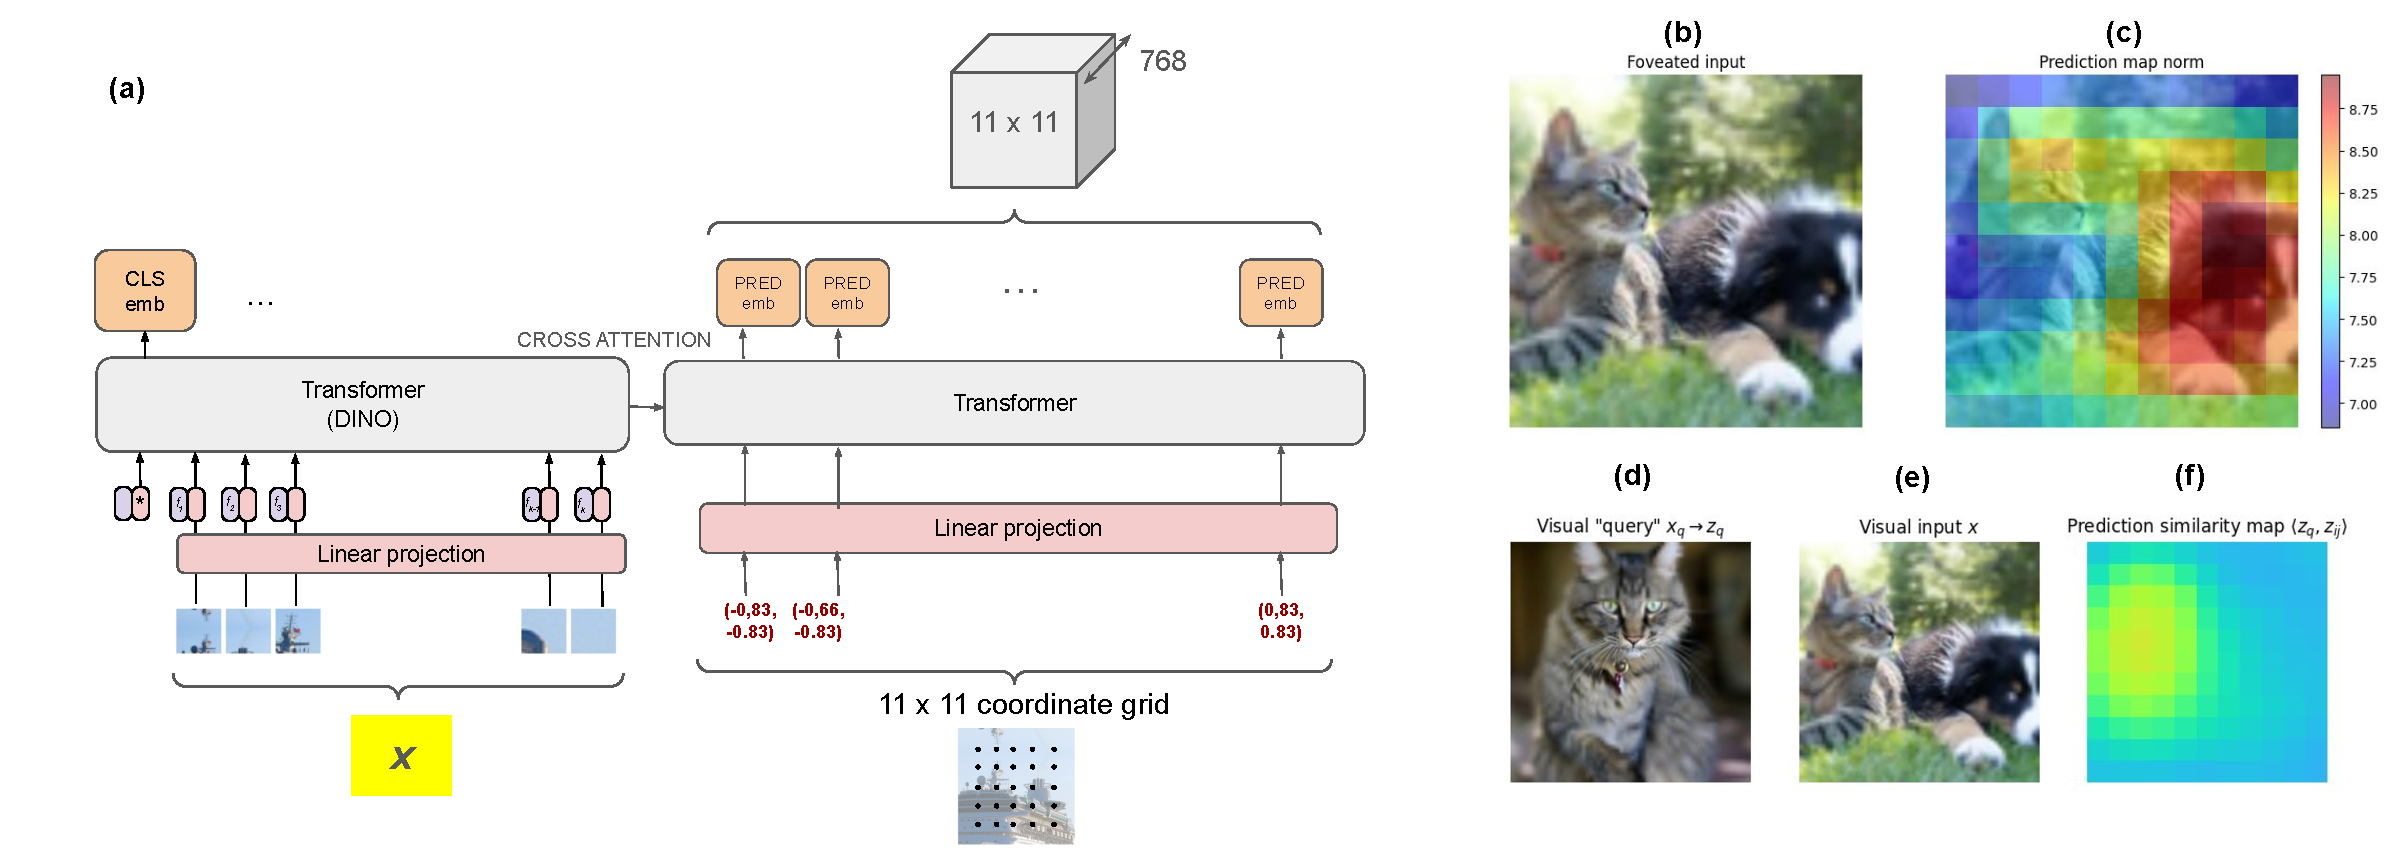
\includegraphics[width=\linewidth]{figs/06_prediction-map.pdf}
  \caption{\textbf{Spatial prediction map}. \textbf{(a)} a spatial prediction map is obtained by parallelizing the predictor's output over a set of coordinates arranged on a regular grid, producing, from a single foveal input, an output tensor of size $11\times11\times768$. \textbf{(b)} example of a foveal image. \textbf{(c)} overlay representation of the norm of the $11\times11$ prediction vectors, color-coded to form a ``saliency'' map. \textbf{(d)} a ``query'' foveal view with a cat at the center of the image. \textbf{(e)} visual input. \textbf{(f)} map of the \emph{cosine similarity} between the query $z_q$ and the prediction grid of vectors $z_{ij}$'s.}
  \label{fig:prediction-map}
\end{figure}

\subsection{Spatial Prediction maps}\label{sec:prediction-map}

The trained model has a forward model capable of predicting a ``future'' feature vector $z'$ from a current view $x$ and a displacement $a$. The transformer architecture makes it straightforward to parallelize this principle to produce multiple predictions from a single view. If we thus define a ``map'' made of a regular grid of eye displacement, relative to the central view, we obtain a prediction extended over the Cartesian space, derived from a single foveal input (see Figure~\ref{fig:prediction-map}).

This results in a feature map of size $11\times11\times768$. An emergent property of our model arises from measuring the \emph{norm} of such predicted vectors. The norm indeed appears to reflect a certain degree of confidence in the resulting prediction, with low-norm vectors corresponding to more uncertain predictions, and therefore more heavily ``penalized'' on average by the MSE loss~\cite{shi2019probabilistic,draganov2025embeddingnorms}. Figure~\ref{fig:prediction-map}c illustrates this, with higher norm values appearing over the most characteristic regions of the two depicted animals, namely the muzzle and the eyes.

A second emergent property appears to be the possibility of \emph{content-based addressing}, in the sense classically introduced by Hopfield~\cite{hopfield1982neural} and more recently reinterpreted through the lens of attention mechanisms~\cite{ramsauer2021hopfield}. We use an image depicting a subject contained in the scene, without requiring an exact match (here, a cat). The encoded image then becomes a ``query'' vector. By measuring the similarity between the query vector and the vectors of the predictive map, it becomes possible to identify the region of the image with the strongest correspondence to the sought-after element, thereby implementing a visual search task~\cite{wolfe2021guided} by \emph{visual correspondence}, i.e. without explicit label.

\subsection{View set}
\begin{figure}[t]
  \centering
  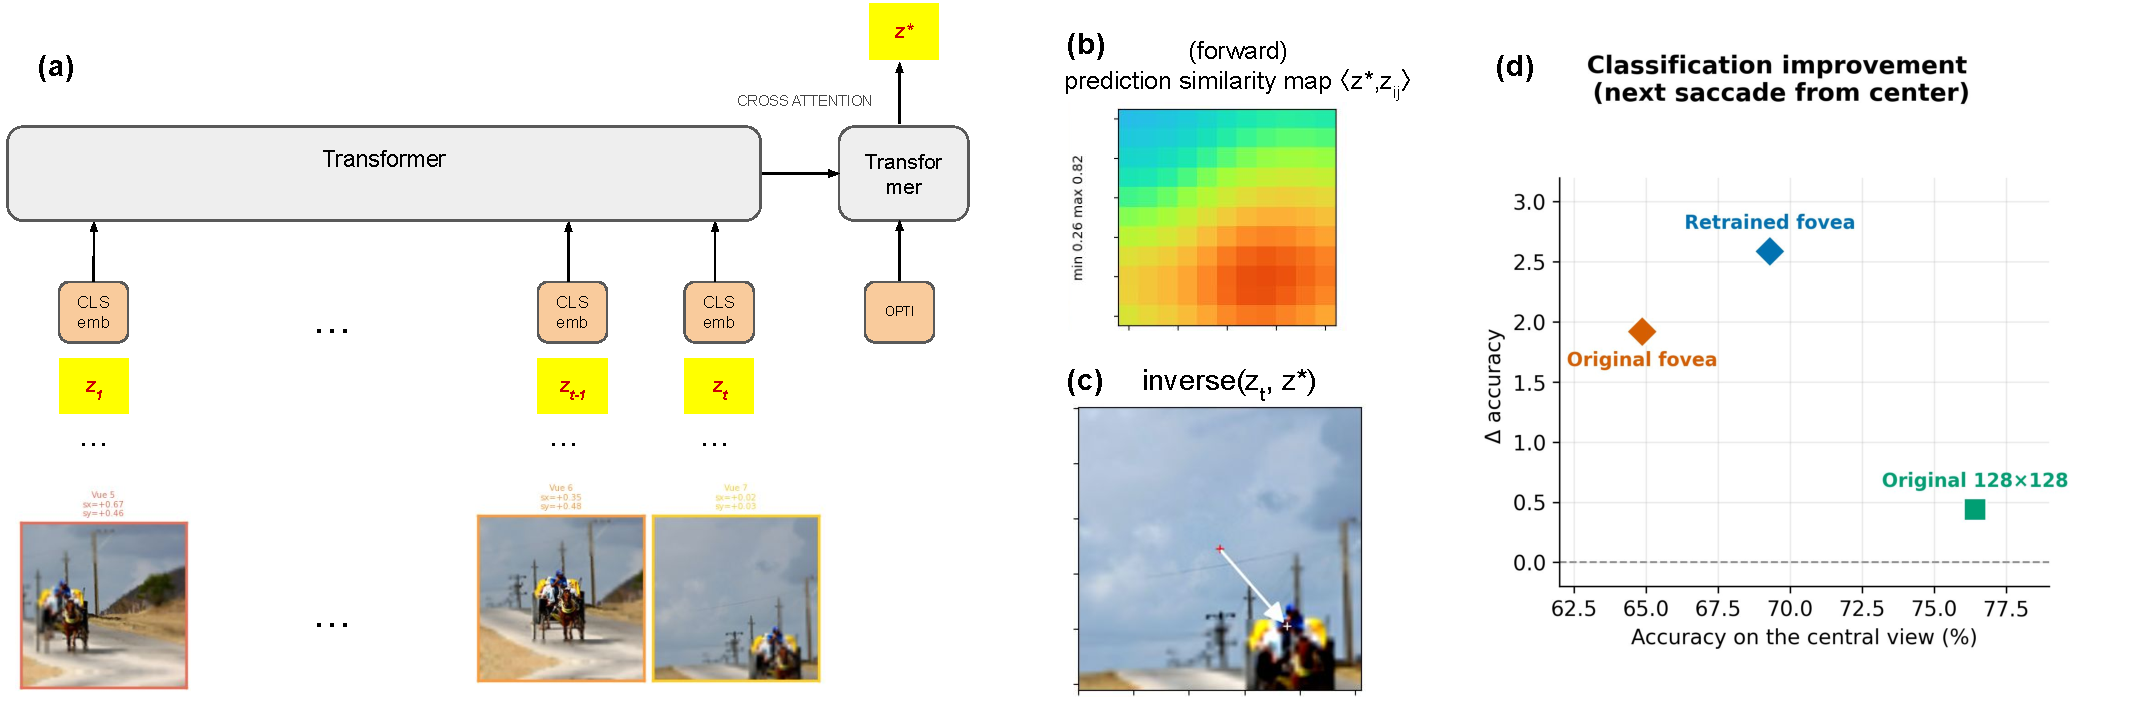
\includegraphics[width=\linewidth]{figs/07_view-set-transformer.pdf}
  \caption{\textbf{Foveal view-set transformer}. \textbf{(a)} a series of saccades is performed over an image. These images are encoded as feature vectors $z_1, \dots, z_t$. A ``lightweight'' two-block transformer processes these vectors as so many ``tokens''. The cross-attention pathway produces a ``target'' token $z^*$. \textbf{(b)} the target token is used as a query to identify the target region through predicted view-map similarity. \textbf{(c)} the inverse model directly produces an eye-displacement command in Cartesian coordinates from $z^*$ and the current view $z_t$.
  \textbf{(d)} Classification improvement compared using the inverse model displacement, on three encoding model: simple 128x128 crops (green), foveal crops without fine tuning (orange), foveal crops with fine-tuning (blue).}
  \label{fig:set-transformer}
\end{figure}


Naturally, a key expected feature of an architecture built around foveal vision is the ability to integrate multiple views of the same visual scene in order to extract holistic, scene-level features. This multi-view integration problem is a classical one, which has been addressed in many different ways~\cite{mnih2014recurrent,cheung2016emergence,dauce2018active,thorat2025predicting,ghaemi2026seq}.

From the standpoint of a natural or artificial vision system, it is important to distinguish the current view, currently being processed by the visual system, from past views, which can be assumed to have been stored in a lightweight or compressed form. 
We consider the scene as encoded in a \emph{set} of views $\{\boldsymbol{z}_1, \boldsymbol{z}_2, \dots, \boldsymbol{z}_k\}$ with \emph{no} explicit spatial indication, assuming the spatial relations between any pair $(\boldsymbol{z}_i, \boldsymbol{z}_j)$ to be computable. 
The order of the views is thus considered irrelevant, consistent with a set-based structure~\cite{lee2019set}.
%Here, we consider past views as being retained in a \emph{set} of representation vectors $z_1, \dots, z_{t-1}$, which we have shown to carry both visual content and positional information.

To demonstrate these integration capabilities, we trained a lightweight, two-block transformer taking as input the encodings of a set of views of the same scene (with no positional encoding). To this end, we created a routine that selects the view that best predicts the target label (in the sense of ImageNet), from a set of 30 randomly cropped views of the same image via the previously trained linear head. The task of the transformer view-set is to predict this ``target'' representation $\boldsymbol{z}^*$ from a set of representations over the same image.  The prediction is done through a cross-attention pathway (see fig~\ref{fig:set-transformer}a), supposedly predicting the most salient view point, or informative element of the image. To train this model, we designate  $\boldsymbol{z}^*$ in a supervised fashion from a set of 30 views. The network takes as input a variable number of ``views'' (between 1 and 15), and is trained on predicting $\boldsymbol{z}^*$.  

%This mechanism works quite well [TO DETAIL]. 
The behaviour of our view set transformer is then tested after training (fig~\ref{fig:set-transformer}, right panel). 
We show that the predicted target representation makes it possible to guess not only the label, but also the relative position of the target object in space. %(more precisely, the object's identification center: typically the muzzle, the eyes, or the head for animals). %We thus obtain an implicit saliency map indicating where to direct the gaze if the task is to identify the content~\cite{itti1998model}.
On fig~\ref{fig:set-transformer}b, we show that $z^*$ can then be used as a ``query'' on the current view, allowing to define a ``saliency'' map via the forward model, like in previous section. Alternately, a 2D vector displacement in the image referential can be computed from the \emph{inverse} model applied on a current representation $\boldsymbol{z}$ and target one $\boldsymbol{z}^*$ (fig~\ref{fig:set-transformer}c). Noticeably, this inverse pathway doesn't require the heavy calculation of a prediction map and should be preferred in a resource-constrained context.

The validity of this displacement in the Cartesian space is difficult to evaluate in the absence of explicit coordinates
for the objects in the ImageNet dataset. Here, we interpret the spatial relevance of the response by
measuring the increase in the classification rate after displacing the eye from the center
with $\boldsymbol{a}^* = \text{inverse}(\boldsymbol{z}_\text{center}, \boldsymbol{z}^*$), where $\boldsymbol{z}_\text{center}$ is the encoding of the central view. We then measure the classification rate at the view reached after the displacement $\boldsymbol{a}^*$, and compare with the one measured at the center. This comparison was made on Imagenet validation set, by training three ``lightweight'' 2-blocks set transformers on different sets of vectors serving as input tokens, coming either from plain or foveal cropped views, and being first transformed either with the original DINO weights or with our finetuned model (fig~\ref{fig:set-transformer}d). The gain of accuracy appears significant for both models including a foveal transformation, but negligible for the one with standard inputs, reflecting once again the absence of usable spatial information in the original DINO [CLS] representations. Interestingly, the foveal transformation alone already yields a surprisingly high gain of +2\%, closely approaching that of our fine-tuned model (+2.5\%). This indicates that, despite the inverse model's lower precision in predicting the shift (see fig~\ref{fig:classif-and-shift} right), some spatial information is yet present in the foveal representation vector, allowing heading in a direction that may improve recognition.

\section{Discussion}

\paragraph{Related work.}
This work belongs to a rapidly growing line of research on learning spatial representations through active exploration of the environment. We discuss below a handful of works that resonate most closely with ours, without claiming exhaustive coverage of this fast-moving area.\begin{itemize}
    \item seq-JEPA~\cite{ghaemi2026seq} conditions a transformer predictor on an action embedding to anticipate the next view's representation, and shows this drives the encoder toward equivariance while an aggregate token stays invariant. It differs from ours in relying on uniform-resolution salient patches rather than genuinely foveated inputs, and in deriving equivariance purely from the forward predictive loss, with no inverse model recovering the action.
    \item Thorat et al.~\cite{thorat2025predicting} train Glimpse Prediction Networks to forecast the next fixation's embedding from the saccadic displacement, and show the resulting representations align with human visual cortex. Their glimpses, however, are full-resolution crops rather than foveated views, their backbone is kept frozen rather than fine-tuned, and the displacement is used only as a forward signal, with no inverse model making space recoverable rather than merely predictable from the representations.
    \item Immonen~\cite{immonen2026action} builds a strikingly similar pipeline on a frozen DINOv2 backbone, with genuine foveation (lowpass-filtered periphery) and an action-conditioned belief transition predicting the next glimpse's token, and shows via ablation that removing action conditioning collapses transition-dependent tasks. Unlike ours, it keeps the backbone entirely frozen and includes no inverse model, casting space instead as belief transitions within a POMDP-style planning agent rather than as a property made recoverable through joint fine-tuning.
    
\end{itemize} 
The objective of this paper was to highlight (1) the lack of spatial content in the feature vectors produced by standard self-supervised architectures, and (2) the central role played by combining a forward model and an inverse model in forcing latent representations to integrate spatial content. The presence of this content makes it possible to leverage powerful predictive mechanisms, associated with ``queries'' or target feature vectors that allow attention to be directed toward regions of interest. Fine-tuning from an already pretrained model shows that it is possible to ``add'' a spatial component to an existing model without destroying the information already present: label information is indeed largely preserved through the fine-tuning procedure.

The key is to understand the constraints that weigh on the redescription space $\boldsymbol{z}$. The DINO encoding provides the richness of the representations, that is, the content of the scene, which must not be degraded. This content was originally trained according to an ``invariance'' logic: two shifted views are supposed to share the same content, which by construction ``erases'' spatial information~\cite{caron2021emerging,chen2020simple}. By fine-tuning DINO with the predictive objective described above, two shifted views of the same scene must be ``sufficiently different'' for the displacement between them to be predictable via the inverse model. We therefore move to an \emph{equivariant} description, without strict geometric constraint ~\cite{cohen2016group}. This is similar in spirit to the SIE approach proposed by \cite{dangovski2022equivariant, garrido2023sie}. Unlike SIE, which prevents collapse to invariance through a dedicated hypernetwork predictor, our mechanism relies on an inverse model recovering the action itself.

The proposed sparse view-set (as opposed to dense, DINOv3-like scene descriptors) is motivated by considerations of biological plausibility. In a highly energy-constrained system such as the brain, it is indeed necessary to retain only the essential content of a scene, in the form of addressable and ``actionable'' content (in the sense of, for instance, a motor displacement toward a target). A major advantage is that the view-set is a very ``synthetic'' description of the visual scene: only a few vectors, hence cheap to store. This is the basic mechanism one would expect in an embedded system where memory must be saved. It is also plausibly what is at work in the brain, where highly compressed versions of past saccades must be retained~\cite{irwin1991information}.

We have here proposed the sketch of a learning model for a latent space that effectively encodes the spatial structure of the surrounding visual environment. It remains a \emph{relative space} rather than an absolute one, since it depends entirely on the movement and displacement capabilities of the agent. 
Learning an \emph{action decoder} (inverse policy), while enforcing the encoding of spatial information, also enables the acquisition of ``how-to-do'' knowledge, namely motor skills and the ability to act upon the world.  

This raises the question of ``objects'', since there is no equivalence between a view and an object. We expect to have shown that, with simple ImageNet labels~\cite{russakovsky2015imagenet}, one can deduce something like the ``position of an object in space'' from a few views that are not necessarily centered on the object. This of course should be confirmed using more specialized object-centric datasets, like  COCO \cite{lin2014microsoft}.
Following the intuition of a dichotomy between \emph{objects} and \emph{space}, as observed in the ventral and dorsal visual pathways of the nervous system, one could also hypothesize a more explicit decomposition of the latent state: $z_t = (c_t, p_t)$, where $c_t$ would reflect the invariant content (the object) while $p_t$ would reflect the equivariant content (the pose).
The effectiveness of our learning procedure nonetheless shows that a mixed position/label content can be deduced from a rather \emph{sparse} set of representations, without a dense embedding \`a la DINOv2 or DINOv3~\cite{oquab2024dinov2,simeoni2025dinov3}.

Furthermore, comparing the representational geometry of our model, via RSA~\cite{kriegeskorte2008representational}, to primate LFP recordings during match-to-sample tasks \cite{fuster1971neuron,miller1996neural} should provide a direct test of whether the spatial code uncovered here has a biological counterpart, narrowing the current gap between the artificial and biological vision systems.

\bibliographystyle{unsrt}
\bibliography{biblio}



\end{document}